\documentclass[12pt]{article}

\usepackage[a4paper,hmargin={2.4cm,2.4cm},vmargin={2.4cm,2.4cm}]{geometry}
\usepackage[mathlines,displaymath]{lineno}
\usepackage{setspace}
\usepackage{amsmath}
\usepackage{amsfonts}
\usepackage{graphicx}
\usepackage[round,colon,authoryear]{natbib}
\usepackage{color, soul}
\usepackage{fancyvrb}
\usepackage{verbatim}
\usepackage[pdftex,colorlinks=true,citecolor=black,linkcolor=black,urlcolor=black,pdftex,pdfstartview=FitH,bookmarks=true]{hyperref}

\bibliographystyle{ecology}



\begin{document}

\title{Improved state-space models for inference about spatial and
  temporal variation in abundance}

\author{Richard B. Chandler  \\
        \small USGS Patuxent Wildlife Research Center \\
        \small Laurel, MD 20708
   \and Jeffrey A. Hostetler \footnote{Contact:
     \url{HostetlerJ@si.edu}, +001-202-633-4205}\\
%        \small Migratory Bird Center \\
        \small Smithsonian Conservation Biology Institute \\
        \small National Zoological Park, MRC 5503 \\
        \small Washington, DC 20013-7012}
\maketitle


\abstract{
Models of population dynamics play a central role in theoretical and
applied ecology where they are used for purposes such as testing
hypotheses about density dependence and predicting species' responses
to future environmental change or management actions. State-space
models are widely used for these purposes because they allow for
estimating parameters of classical growth models, such as exponential,
logistic, and Gompertz, while accounting for demographic stochasticity
and observation error. Conventional state-space models, however, have
three important limitations: (1) the parameters are not identifiable
in many common situations, (2) they do not admit spatial variation in
population dynamics, and (3) there is no clear interpretation of the
observation error. We demonstrate how each of these problems can be
resolved using a class of hierarchical models for spatially-replicated
time-series data recently proposed by
\citet[Biometrics]{dail_madsen:2011}. We
expand this class of models to accommodate classical growth
models, zero-inflation, and random effects such as observer-specific
detection probabilities. Furthermore, we describe classical and
Bayesian methods of parameter estimation. These new developments will
allow researchers to apply these methods to address important
questions regarding the factors affecting spatial and temporal
variation in abundance. We demonstrate these developments by analyzing
data from the North American Breeding Bird Survey. Code to fit these
models using the \textbf{R} package \texttt{unmarked} and
\textbf{JAGS} is also provided.
}

\vspace{0.5cm}

\textbf{Key words}: abundance, Dail and Madsen model, density-dependence,
Gompertz model, immigration, open population point count models,
random observer effects, range, Ricker model, zero-inflated

\newpage

Theoretical ecology requires models of population dynamics for testing
hypotheses regarding spatial and temporal variation in
abundance---hypotheses relating to the importance and existence of
phenomenon such as density-dependent population regulation, population
cycling, and spatial synchrony
\citep{royama:1977,turchin:1990,dennis_taper:1994,bjornstad_etal:1999}.
%growth ,viljugrein_etal:2005}.
In applied contexts, population models are used for %population viability
%analysis, including the estimation of
estimating extinction probabilities
\citep{nadeem_lele:2011} and for predicting the effects of future
environmental conditions or conservation actions on population size
\citep{jamieson_brooks:2004}.
%Such models are
%also required in applied ecological research
%for predicting species' responses to environmental change or
%conservation actions. For example, %many researchers are currently
%models of population dynamics allow for inference about the effects of
%of climate change on population viability.
%investigations of the influence of climate on population dynamics so that
%predictions can be made about the effects of climate change.
In order to address these questions, several complicating factors must
be confronted when fitting population models to data.
First, deterministic models of population
dynamics are virtually always inadequate due to process variation,
the inherent stochasticity in demographic parameters and environmental
conditions \citep{bjornstad_grenfell:2001}. %clark_bjornstad:2004}.
Second, abundance---the natural state variable in studies
of population dynamics---can rarely be observed perfectly in field
studies because of observation error, such as imperfect
detection \citep{kery_etal:2009}. Failure to account for process
variation and observation error can bias the estimators of abundance
and related parameters.

State-space models are a widely used approach for
studying population dynamics while accounting for process variation
and observation error \citep{devalpine_hastings:2002,
  buckland_etal:2004, dennis_taper:1994,
  dennis_etal:2006}. Conventional state-space models are
simply time-series models in which the true state of the system
(e.g. population size during each year) is
observed imperfectly. Originally developed for xxx (cite Kalman filter
papers), the ability to model both the ecological state process and
the observation process has made them relevant in numerous ecological
applications [need to clean this up]. State-space models have been
defined differently by different authors, but we follow
\citet{buckland_etal:2004} the definition : ``xxx'' . Typically, the
ecological
process is described by a Markovian model that includes a
deterministic description of population change as well as two random
sources of variation for ``process variation''. The model for the
observation process is typically phenomenological in the sense that
observation error is not defined explicitly. As an example, let $N_t$ be
the abundance of a species during year $t$, and $X_t$ be the observed data,
which differs from  due to observation error ($\zeta$). A simple state
space model that includes exponential growth and process variation
($\grave{o}$) could be written as:
\begin{gather}
N_t = N_{t-1}\exp(r)+\grave{o}_t \nonumber \\
X_t = N_t + \zeta_t
\end{gather}
Here   is the intrinsic rate of increase. Typically, both random
effects are assumed to follow normal distributions: $\grave{o}_t \sim
\mathrm{N}(0, \sigma)$ and $\zeta_t \sim \mathrm{N}(0, \tau)$
\citep{devalpine_hastings:2002,dennis_etal:2006}. Even though this is
the most widespread approach for modeling population dynamics using
time-series data, several problems are immediately evident. First, if
abundance is a non-negative integer, as it always is, there is clearly
a problem with this formulation because the normally distributed
random effects violate this constraint. To avoid this issue,
ecologists often replace $N_t$ with $\log(Y_t/A)$   where $A$ is the
area surveyed---i.e.,
abundance is replaced by the natural log of population density, which
is assumed to normally distributed. This is desirable because this
allows for the fitting of models assuming normally distributed
residuals, which are computationally much less intensive than most
alternatives. However, this transformation is problematic since
abundance may be zero and thus $Y_t = \log(0) = -\infty$. Generally,
zeros are replaced with
some small, but positive number, although the effect of this is rarely
discussed.

The problems mentioned thus far are minor in comparison to the more
serious issue that the parameters of the model are often not
identifiable. Specifically, the Markovian nature of the model implies
the following likelihood
\[
LIKELIHOOD
\]
The first term is the probability density for the first observation in
the time series, $Y_t$, yet it is intuitively not possible to estimate the
parameter(s) of this distribution using only a single
observation. This problem has resulted in several papers with
interesting names like ``multi-modal likelihoods and ridges etc...''
The workaround here is to assume that the population is at equilibrium
so that that the x can be replaced with the equilibrium
distribution. However, assuming equilibrium defeats the objective of
many studies of population dynamics, namely determining if and why a
population is at equilibrium.

A third problem with these models is that they do not admit
spatial variation. This is not a fair criticism because this
lies beyond the scope of traditional state-space models, but
it does restrict the utility of their since it is typically
impossible assess the impacts of factors such as habitat
fragmentation or climate change on a population without
considering spatial variation. Indeed many populations are
regulated by spatial processes such as source-sink dynamics.

\citet{dail_madsen:2011} developed a model (henceforth the DM model)
that resolves each of these problems with traditional state-space
models. The DM model allows for inference about spatial and temporal
dynamics in abundance while accounting for observation error using
only spatially and temporally replicated count data.  Their model is
an extension of the closed-population N-mixture model
\citep{royle:2004biom}, which was designed specifically to address the
problem of
modeling spatial variation in abundance when detection probability is
less than unity. The DM extension relaxes the assumption of population
closure and includes explicit parameters describing population change
as a first-order Markovian process. [more details]

[applications / potential etc... ] The DM model is relevant to a huge
number of problems confronting basic and applied ecological
research. Answering questions about climate change etc... require
spatially and temporally extensive datasets such as result from the
North American Breeding Bird Survey (BBS)
\citep{robbins_etal:1986}. However, most of the datasets of the
appropriate scale are
collected by volunteers and using protocols that are not amenable to
traditional approaches of modeling abundance and detection probability
based on standard capture-recapture methods. Instead they have, at
best, simple count data for which, when it can be interpreted as
counts of unique individuals, the DM model can be applied.. Yadi ya

Although the DM model was designed explicitly for these purposes, the
original formulation of the model makes strict distributional
assumptions and does not acknowledge many of the sources of variation
inherent to existing ecological time-series data.  We propose
variations on these models that are likely to be more realistic and
useful in many cases.  We demonstrate the usefulness of these new
models with simulated and real BBS data.


\section{Model Development}

\subsection{Original Formulation}

As originally formulated, the DM model includes submodels for four
conditionally related processes: the initial abundance state, apparent
survival, recruitment, and detection probability. \citet{dail_madsen:2011}
proposed two distributions for initial abundance, the Poisson and negative
binomial:
\begin{gather}
N_{it} \sim \mathrm{Pois}(\Lambda) \nonumber \\
N_{it} \sim \mathrm{NB}(\Lambda, \alpha)
\label{eq:N1}
\end{gather}
where $N_{i1}$ is the abundance at site $i=1,\hdots,R$ during year 1
and $\Lambda=\mathbb{E}[N_{i1}]$ is the expected abundance. The negative
binomial model includes the overdispersion parameter $\alpha$.  The
survival and recruitment terms allow abundance to change over time:
\begin{equation}
\left.\begin{aligned}
S_{it}|N_{it-1} &\sim \mathrm{Bin}(N_{it-1}, \omega) \\
G_{it}|N_{it-1} &\sim \mathrm{Pois}(\gamma(N_{it-1})) \\
N_{it} &= S_{it}+G_{it}
\end{aligned}\right\} \quad \text{for} \; t=2,\hdots,T
\label{eq:Nt}
\end{equation}
where $\omega$ is the survival probability and $\gamma$ is the arrival
rate (which can depend on $N_{it-1}$). Dail and Madsen propose three models
for $\gamma$: the constant model, where $\gamma$ does not depend on
$N_{it-1}$, and which simulates a ``propagule rain'' of recruitment; the
autoregressive model , which
simulates geometric or density independent growth; and the ``no-trend''
model, which keeps abundance fixed over time.

Eqs.~\ref{eq:N1} and \ref{eq:Nt} fully specify the state model---the
model for spatial and temporal variation in abundance. The observation
model assumes that individuals are missed due to imperfect
detection. The simplest model for imperfect detection is
\begin{equation}
  n_{it} \sim \mathrm{Bin}(N_{it}, p)
  \label{eq:p1}
\end{equation}

Initial abundance, apparent survival, recruitment, and detection can
all be modeled as functions of covariates, allowing fairly
sophisticated inference about population processes and dynamics from
point count data.

\subsection{Range model of initial abundance}

\citet{dail_madsen:2011} suggested two distributions for modeling
initial abundance: Poisson and negative binomial.  We have extended
their model to include another distribution, the zero-inflated
Poisson.  This could be useful when, for example, one is modeling the
abundance of several bird species with the same set of BBS routespoint
count surveys for all species, but this set includes routes sites
outside the range of some of the bird species.  The distribution of
initial abundances can be represented as:
\begin{equation}
N_{i1} \sim \left\{
\begin{aligned}
0 &\; \text{with probability} \; \psi \\
\Lambda &\; \text{with probability} \; (1-\psi)
\end{aligned} \right.
\label{eq:ZIP}
\end{equation}
where $\psi$ represents the proportion of extra zeros.

These models allow three sources of zero counts by observers: a
species was at a route but not detected; the route was within the
species' range but there were no birds at that site in that year; and
the route was outside the species' range.  Furthermore, detection,
abundance, and zero-inflation can be modeled separately as functions
of different (or the same) covariates.  For example, detection of
species x at site y in year z might depend on wind speed, abundance on
forest type and weather, and zero-inflation upon elevation and
climate.  This approach combines elements of occupancy modeling
\citep{mackenzie_etal:2006} and abundance modeling.
%, and could prove useful
%for distinguishing species' fundamental and realized niches
%(Hutchinson 1957).

The zero inflation factor can also affect
recruitment or population dynamics (see below).
We also considered a zero-inflated negative binomial model of initial
abundance, but this model did not perform well in preliminary tests.

\subsection{Population growth models}

Preliminary DM model runs for several species tended to lead to
estimates of survival that were unrealistically high and recruitment
that were unrealistically low, or the reverse (compared to independent
demographic analyses).  The DM models are able to partition changes in
abundance to survival and recruitment in part by making strong
distributional assumptions. % (Dail and Madsen 2011).
When those assumptions are heavily violated the models may proportion
population growth incorrectly into survival and recruitment, even if
they estimates population growth accurately.

Although partitioning population growth into survival and recruitment
is informative, it is not needed for all applications.  Furthermore, a
simpler model would have several merits: faster running time, fewer
total model combinations, and possibly more realistic estimates.
Therefore, we developed a version of the DM model that estimates and
models population growth directly.  In this model, Eq.\ref{eq:Nt} is
simplified to:
\begin{equation}
  N_{it} \sim \text{Pois}(\exp(r)N_{it-1})
\label{eq:exp}
\end{equation}
where $r$ represents the instantaneous population growth rate.  This,
like the autoregressive version of the model, is a variant on a simple
density-independent exponential model of population growth.
Density-dependent versions of the model are also possible.  For
example:
\begin{equation}
  N_{it} \sim \text{Pois}(N_{it-1}\exp(r(1-N_{it-1}/K))
\label{eq:rick}
\end{equation}
where $K$ is the stable equilibrium of the population and $r$ is the
instantaneous population growth rate at low population densities, and
both parameters are constrained to be positive.  This model is based
on the \citet{ricker:1954} discrete time version of the logistic population
growth model.  We also implemented the \citet{gompertz:1825} density-dependent
model:
\begin{equation}
  N_{it} \sim \text{Pois}(N_{it-1}\exp(r(1-\log(N_{it-1})/\log(K)))
\label{eq:gomp}
\end{equation}
where the log of $N_{it-1}$ is only taken when $N_{it-1}>0$
(when $N_{it-1} \equiv 0$, the full expression simplifies to 0 anyway).  Here
the interpretations of $r$ and $K$ are similar to in the Ricker model, but
$K$ is constrained to be greater than one.

Because a single Poisson distribution controls the
distribution of $N_{it}$ in each of these models, the discrete
convolution used by \citet{dail_madsen:2011} is not required,
speeding up processing time.

\subsection{Immigration models}

The autoregressive, population growth, Ricker, and Gompertz
versions of the DM models all share a common feature (or bug):
once the population at a site reaches 0, it must remain at 0.
This is because all contributions to population growth are
local in these models.  We generalized each these models that
include both internal and external (immigration) contributions
to population growth.  The population growth plus immigration
model is:
\begin{equation}
  N_{it} \sim \text{Poisson}(\exp(r)N_{it-1}) + \text{Poisson}(\iota)
  \label{eq:expimm1}
\end{equation}
or equivalently
\begin{equation}
  N_{it} \sim \text{Poisson}(\exp(r)N_{it-1} + \iota)
  \label{eq:expimm2}
\end{equation}
where $\iota$ represents the immigration rate.  This model is close to
the constant DM model (equation 4), with $\exp(r)$ instead of $\omega$
and $\iota$ instead of $\gamma$, except that the first
process is Poisson distributed instead of binomial. The Ricker and
Gompertz models can be extended to allow for immigration in the same
way.
\begin{comment}
  Similarly, the Ricker + immigration model can be represented as: the
  Gompertz + immigration model as: (13) and the autoregressive +
  immigration model as: (14)
\end{comment}

% Save for discussion
\begin{comment}
  These immigration models are based on the assumption that number of
  immigrant is not dependent on local density; however, extending
  these models in this way is conceptually straight-forward, a Other
  versions of these models with different assumptions are
  possible. The Ricker + immigration and Gompertz + immigration models
  can be justified by the further assumption that immigrants arrive as
  adults immediately before the point-count survey (so that
  density-dependent processes do not have a chance to act on the
  numbers of immigrants; Otto and Day 2007 p. 161).  Deterministic
  versions of these models do reach stable equilibriums, but the
  equilibriums are not at K and cannot be solved for analytically
  (Otto and Day 2007).
\end{comment}

We have implemented all preceding models in
a maximum likelihood framework by extending the \texttt{unmarked} package
\citep{fiske_chandler:2011} in \textbf{R} \citep{R-2012}.

\subsection{Random effects of observers}

Differences in observers' ability to see, hear, or identify
birds has long been recognized as a potential source of error
in avian point count surveys such as the BBS
\citep{robbins_etal:1986,diefenbach_etal:2003,sauer_etal:1994auk,alldredge_etal:2007auk,campbell_francis:2011}.
Estimating a separate detection probability for each observer can be
difficult and reduces one's ability to estimate the quantities
of interest.  This problem is compounded by the fact that
observers differ greatly in the number of surveys they have
run (so that many observers' separate detection probabilities
could not be accurately estimated).

Current BBS trend estimators deal with this problem by
treating observer identity as a random (as opposed to a fixed)
effect \citep{link_sauer:2002,sauer_link:2011}.
%(Link and Sauer 2002, Sauer and Link 2011).
This allows observer-specific differences in detection probability,
but assumes that observers are selected at random from a pool
of potential observers.  Models that contain both random and
fixed effects are referred to as mixed models.  Often in mixed
models (as in this case), the random effect is modeled not
because it of interest in itself, but to avoid bias in the
estimates of the fixed effects.

To include random observer effects in DM models and these extensions,
Eq.~\ref{eq:p1} can be modified to:
\begin{gather}
n_{ijt} \sim \mathrm{Bin}(N_{it}, p_j) \nonumber \\
\mathrm{logit}(p_j) \sim \mathrm{Normal}(\mu_p, \sigma_p)
\label{eq:pobs}
\end{gather}
where $n_{ijt}$ is the number of bird recorded at site $i$ by observer $j$ in
year $t$, $p_j$ is observer-specific detection probability, $\mu_p$ is the mean
detection probability (on the logit scale), and $\sigma_p$ is the standard
deviation of the random observer effects (also on the logit scale).
We have implemented random observer effects in the Bayesian framework
using program \textbf{JAGS} \citep[version 3.2.0]{plummer:2003}
% (version 3.2.0; Plummer 2003)
with the \textbf{R} (R
Development Core Team 2011) package \texttt{rjags} \citep{plummer:2011}
%(Plummer 2011)
interface.

\subsection{Dynamic range models}

The zero-inflated Poisson distribution can be applied to not only
initial abundance but also to recruitment and population growth terms.
For example, the recruitment term of the constant DM model (equation
4) can be modified as follows:
\begin{equation}
G_{it} \sim \left\{
\begin{aligned}
0 &\; \text{with probability} \; \psi \\
\mathrm{Poisson}(\gamma) &\; \text{with probability} \; (1-\psi)
\end{aligned} \right.
\label{eq:ZIPts}
\end{equation}
When both initial abundance and dynamics are modeled as zero-inflated,
$\psi$ can be modeled as time-varying or not (in either case, $\psi$ can also be
modeled as varying over space).  In the latter case, it makes sense
for the model to "remember" which sites are inside the range of the
species between the initial abundance stage and each time step of the
dynamics stage (see code sample?).  Adding zero-inflation to the
dynamics of the autoregressive, trend, Ricker, or Gompertz models
(without immigration) should have no effect when initial abundance is
also zero-inflated unless $\psi$ is time-varying (because these dynamic
models cannot recover from zero abundance).  We have implemented
zero-inflated dynamics in the Bayesian framework using program
\textrm{JAGS} \citep[version 3.2.0]{plummer:2003}.
%(version 3.2.0; Plummer 2003)


\section{Applications}

\subsection{Simulation Study}


We simulated data for 100 sites over 40 years.  All
simulations assumed initial abundance was Poisson distributed
and no covariates affected initial abundance, dynamics, or
detection probability.  Our first series of simulations
assumed dynamics were exponential.  We ran 1000 simulations for
each combination of low, medium, and high $\Lambda \in \{1,5,10\}$, $r
\in \{-0.005, 0, 0.005\}$, and
$p \in \{0.05, 0.25, 0.5\}$. % (Table 1; 27 total combinations).

Our second series of simulations changed dynamics to the
Ricker model.  We used an initial abundance of 10, a maximum
growth rate of 0.005, and a detection probability of 0.25, and
simulated low, medium, and high values of equilibrium
abundance, each with 500 simulations (Table 1).  Our third
series of simulations was based on the Ricker + immigration
dynamics model; here we fixed all parameters the same as the
Ricker model (with K = 10) and simulated low, medium, and high
values of immigration rate with 500 simulation each (Table
1).

We estimated the parameters for each simulation using the same
initial abundance (Poisson) and dynamics models as were
simulated, implemented in the unmarked library in \textbf{R}.  When run
in a maximum likelihood framework, these models require a
maximum abundance to integrate over
\citep{royle:2004biom,dail_madsen:2011};
%(Royle 2004, Dail and Madsen 2011);
we used 200.  We report bias of estimates, root
mean squared error, and coverage (percentage of 95\% confidence
intervals for parameters that
overlap the true values).

Ideas:
I.	Test importance of random effects modeling, and other differences between JAGS and unmarked
II.	Model with low p values, or a range of p values
III.	Ability to distinguish correct initial abundance and dynamics models
IV.	When can you detect DD if it exists (power)?
V.	Building on the last two: what if your model set doesn't
include the correct DD model?  When will the wrong DD model be favored
over the wrong DID model?



\subsection{Analysis of Breeding Bird Survey Data}

We applied these models to North American Breeding Bird Survey (BBS)
data from 1966-2010 for two species in the bordering US states
Maryland and Virginia.  For our focal species, we selected ovenbirds
(\textit{Seiurus aurocapilla}), an abundant and widespread forest breeding
migrant with a stable or increasing trend in the region (CITE) and
golden-winged warblers (\textit{Vermivora chrysoptera}), which only breeds in
the western parts of these states and has been declining in the region
(CITE).  MORE INFORMATION ABOUT THE SPECIES?

GENERAL ABOUT BBS DATA.  We only used data marked as acceptable for
use in the annual BBS analysis.  We summed the total birds of each
species seen on each route and year and used the routes (rather than
the individual stops) as our sites.
Strong winds can interfere with point count observers' ability to hear
birds (\citep{simons_etal:2007}); we tested the effects of wind speed
on detection probability.  BBS volunteers record wind conditions at
the beginning and end of each route on the Beaufort Scale
\citep[start and end wind 0-9]{robbins_etal:1986}.
%(start and end wind; Robbins et al. 1986)(start and end wind; 0-9; cite).
When
start or end wind was not recorded we imputed those values with the
start or end mean.  We took the mean of start and end wind for each
route and put this average wind scale value into four categories: 0 $\leq$
wind $<$ 1; 1 $\geq$ wind $<$ 2; 2 $\leq$ wind $<$ 3; and wind $\geq$ 3 (maximum of 3.5).
Following \citet{link_sauer:2002},
%Link and Sauer (2002),
we also included the first time an
observer ran a route as a predictor variable for detection
probability.

HOW WE OBTAINED AND MANIPULATED PRISM DATA
We ran a series of maximum-likelihood based models for each species,
and then a series of Bayesian models.  We started by testing three
models of initial abundance (Poisson, negative binomial, and
zero-inflated Poisson) with population growth dynamics (equation 7)
and no covariates.  We selected the minimum Akaike's Information
Criterion (AIC) model from that set to test three additional models
for p: wind, first, and wind + first.   We selected the minimum AIC
model from that set to test eight additional models of dynamics:
constant, autoregressive, Ricker, Gompertz, autoregressive +
immigration, population growth + immigration, Ricker + immigration,
and Gompertz + immigration.  We then tested the effect of average
minimum temperature for June and July on all dynamics parameters from
the minimum AIC dynamics model.  When run in a maximum likelihood
framework, these models require a maximum abundance to integrate over
(Royle 2004, Dail and Madsen 2011); we used 600 for ovenbirds and 350
for GWWA.

We ran the top ranked models from the maximum likelihood analyses in a
Bayesian framework.  We added random observer effects and, where
appropriate, zero-inflated dynamics.  WILL ADD MORE HEREWe used
non-informative priors.  We tested for lack of convergence using X
Markov chains for each model \citep{gelman_rubin:1992}.
%(Gelman and Rubin 1992).
For each chain
we sampled the MCMC for Y iterations, after Z tuning samples.  Latent
inclusion factors for temperature effects?

\section{Results}

The negative binomial distribution was strongly supported for ovenbird
initial abundance over the Poisson and zero-inflated Poisson (Table
1A, models A.1 - A.3).  Even compared to the Poisson, there was no
evidence to support a zero-inflation factor for this species.  The
best supported model for p was additive effects of wind speed and
first run (Table 1A, model A.4).  First run and increasing wind speeds
both decreased p.  All dynamics models with immigration were better
supported than models without immigration (Table 1A, models A.8 -
A.16); the best supported of these was the Ricker + Immigration.  The
best supported model of those without immigration was the Gompertz,
and the autoregressive and the constant model had the least support.
There was little support for an effect of minimum June and July
temperature on dynamics parameters of the Ricker + Immigration model
(Table 1A, models A.17 - A.18).

Estimates for the top ranked model for OVEN
(NB[$\Lambda (.) \alpha (.)$]Ricker+Imm.[$r(.)K(.) \iota (.)$]p(wind+1st)) were similar when
run in the Bayesian framework, except that the estimate of r more than
halved (from 0.026 $\pm$ 0.006 to 0.011 $\pm$ 0.005 [for Bayesian model
estimates we present mean and SD]).  When random observer effects were
added, estimates for $\Lambda$ and K increased dramatically (from 31.6 $\pm$ 4.9
to 42.5 $\pm$ 7.3 and from 56.2 $\pm$ 18.2 to 101.8 $\pm$ 21.1, respectively), and
the estimate for r was intermediate (0.018 $\pm$ 0.006).  The estimate of
the intercept for p (on the logit scale) dropped from -1.5 $\pm$ 0.1 to
-2.0 $\pm$ 0.1, and the estimate of $\sigma_p$ was 0.35 $\pm$ 0.03.  [Richard, I ran
the temperature model in the Bayesian framework (w/ and w/o random
effect) too.  Should we include those results?  As earlier, very
little evidence for an effect of temperature on any of the parameters,
although I couldn't get the latent inclusion parameter to work for r.]
Gelman and Rubin diagnostics and visual examination of the ? plots
provided some evidence for a lack of convergence in estimates of the
intercept for p for all Bayesian models ran.

There was slightly more support for the ZIP distribution for initial
abundance of GWWA than for the negative binomial; both were strongly
supported over the Poisson (Table 1B, models B.1 - B.3).  The best
supported model for p was an effect of first run (Table 1B, model
B.4).  The best supported dynamics model was population growth (Table
1B, model B.8); the estimate of r from this model was -0.058 $\pm$ 0.017
(SE).  There was no support for immigration added to the population
growth or autoregressive models (Table 1B, models B.10 and B.13).
However, the Gompertz + immigration and Ricker + immigration models
were supported over the corresponding models without immigration
(Table 1B, models B.11, B.12, B.14, and B.15), despite low estimates
of $\iota$ from these models (0.003 $\pm$ 0.003 and 0.003 $\pm$ 0.002,
respectively).  There was considerable support for an effect of
average minimum June and July temperature on r in the population
growth model (Table 1B, model B.17), with a negative slope.

Because of the closeness of rankings for the ZIP and negative binomial
distributions for GWWA, we also ran the subsequent models with the
negative binomial initial abundance.  Rankings of subsequent models
were similar, but with a p covariate (first) the negative binomial
distribution outranked the ZIP.

STILL WORKING ON JAGS GWWA RESULTS
Estimated detection probabilities were generally low.  For OVEN, the
estimated probability of detecting a bird with no wind and not the
first time an observer had run a route varied between 0.046 $\pm$ 0.002
(model A.16) and 0.192 $\pm$ 0.015 (model A.11), among models that
accounted for both.  For GWWA, the estimated probability of detecting
a bird by a non-first time observer varied between 0.025 $\pm$ 0.008
(model B.18) and 0.141 $\pm$ 0.027 (model B.16), among models that
accounted for first but not wind.

For both species, constant dynamics models estimated very high
survival probabilities ($\omega$ = 1 $\pm$ 1.3e-05 for OVEN and 0.935 $\pm$ 0.011 for
GWWA).   The autoregressive and autoregressive + immigration models
estimated very low survival probabilities for OVEN ($\omega$ = 0.058 $\pm$ 0.046
and 0.026 $\pm$ 0.060, respectively), but not for GWWA ($\omega$ = 0.715 $\pm$ 0.288
for both models).



\begin{figure}
  \centering
  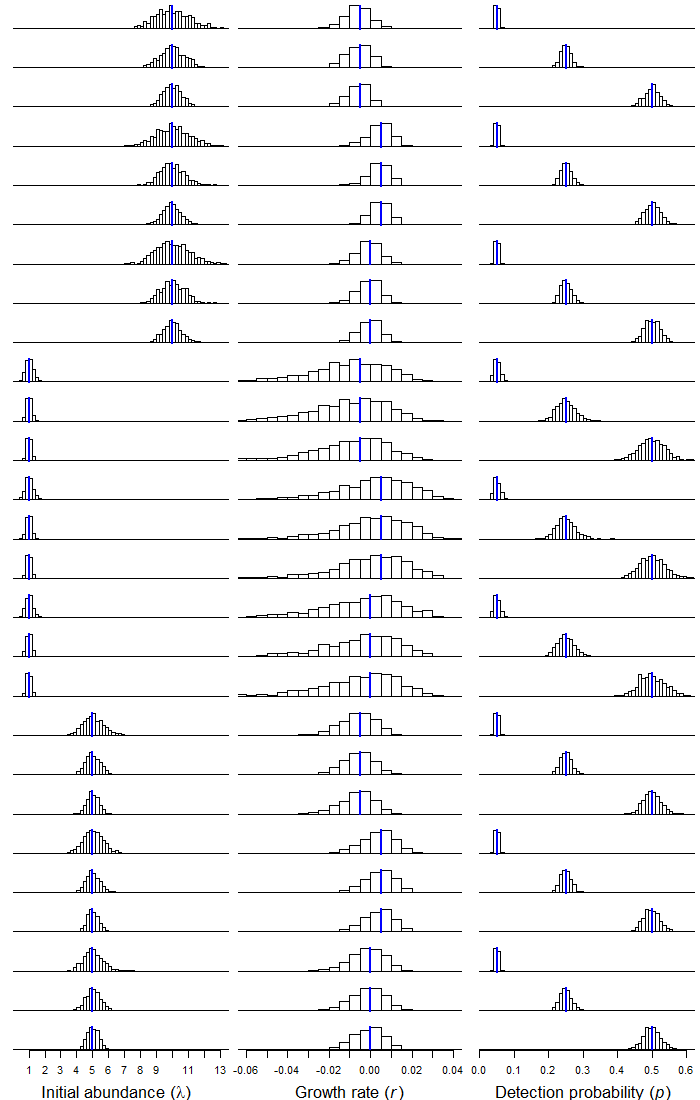
\includegraphics[height=8in]{figs/exp_hists}
  \caption{Histograms of 1000 parameter estimates for each of 27 simulation cases. The verticle lines are the data-generating values.}
\label{fig:exp_hists}
\end{figure}

\section{Discussion}



We made four important developments of the open population
N-mixture model proposed by Dail and Madsen that make the
model more applicable to long-term data such as is collected
by the North American Breeding Bird Survey. First, we have
reconciled the objectives of traditional state-space models
with open population N-mixture models by illustrating how
classical models of population dynamics can be embedded within
the framework. Second, we have demonstrated methods of
accounting for zero-inflation in the time-series. Third, we
have illustrated how additional random effects such as
observer-specific detection probabilities can be
accommodated. Fourth, we presented a Bayesian analysis of the
model, which makes it much easier to estimate parameters and
to fine tune the model for specific purposes.

A unique aspect of the Dail and Madsen model as originally devised was
that it allowed for the estimation of demographic parameters under
strict distributional assumptions and with the assumption of
geographic closure. Clearly, estimating demographic parameters from
count data is a loftyn ambitious goal, and the required assumption
will not be valid in many cases. Nonetheless, their approach is
important because it allows for the combination of count data with
other data types such as capture-recapture data , which offers a
means of making inferences about demographic processes at broad
spatial scales. Models combining count data and demographic data are
often referred to as integrated population models, and This topic has
received much attention lately under t

In the absence of direct information about demographic parameters, and
when the original assumptions of the model do not hold, we have
offered extensions of the model to estimate derived parameters such as
population growth rate. This has been the traditional emphasis of
state-space models, and our approach resolves many of the factors
limiting ...

[paragraph on zero-inflation]The zero-inflated models for initial
abundance and dynamics allow one to estimate and model the proportion
of sites outside of the range of a species.  This could be especially
useful when different factors control the range than the abundance or
dynamics within the range.  [some examples where that is the case?]

[paragraph on random effects]
[paragraph on Bayesian]
In spite of the new extensions we have proposed, several aspects of
the model could be improved. First, the precision with which the
parameters of the state process can be estimated ultimately depends
upon how well detection probability is estimated. When there is only a
single survey per primary period, the information about detection
probability comes from deviations from the parametric assumptions
about population dynamics. Thus, without direct information about
detection probability, the estimates will be determined by model based
assumptions. Furthermore, there are multiple components of detection
probability that should be accounted for to minimize bias and yield
valid estimates of population size. [Nichols EURING paper] .

Fortunately, it is easy to incorporate direct information about
detection probability and we recommend that this be done whenever
possible. The original method for proposed in the original paper was
to collected replicated counts within the primary periods during a
period in which the populations could be assumed to be closed.  a
robust design could be used to combine multiple surveys per primary
period to increase the precision of the estimates. We envision that
multiple other options are available as well. For instance, there
should be no difficulty extending the model to accommodate traditional
capture-recapture data collected during each primary period. Removal
or time of detection etc.. Distance-related heterogeneity in detection
probability is another source of variation that can bias estimators of
abundance.   Show some equations for the alternative observation
models.

[paragraph on spatially-explicit dispersal]
[Other possible extensions we could mention:
Spatially hierarchical model (so can use individual stops)
Other models of variability in growth or recruitment (such as negative binomial)
Add density dependence to survival and recruitment models]
[Discuss causes of low p values (and other BBS results) here or in BBS
results?]

The modeling framework we described can be used to address many of the
most pressing issue in ecology and conservation biology. For example,
it is possible to test hypotheses about temporal and spatial
population regulation. Furthermore, the Bayesian approach is very
useful in that it can be used to combine multiple sources of data to
develop mechanistic models of population dynamics. Thus one can test
hypotheses about the effects of climate change on either explicit
demographic parameters or in derived parameters such as population
growth rate. Furthermore, under the Bayesian approach , population
viability analysis is trivial because projecting populations into the
future can be done as a component of the MCMC analysis. This allows
for the computation of posterior distributions of parameters such as
quasi-extinction probability.




\bibliography{Dail_Mad_ext}

\end{document}
